\documentclass[aspectratio=1610]{beamer}

\usepackage[utf8]{inputenc}
\usepackage{graphicx}
\usepackage{amssymb}
\usepackage{enumitem}
\usepackage[export]{adjustbox}
\usetheme{Frankfurt}
\usefonttheme[onlymath]{serif}

\graphicspath{{./Figures/}}

\definecolor{satinsheengold}{rgb}{0.85, 0.63, 0.21}
\setbeamercolor{structure}{fg=satinsheengold}
\setbeamercolor{title}{fg=black}
\setbeamercolor{title in head/foot}{fg=black, bg=satinsheengold}
\setbeamercolor{author}{fg=black}
\setbeamercolor{frametitle}{fg=black}
\setbeamercolor{author in head/foot}{fg=black, bg=satinsheengold}
\setbeamercolor{institute in head/foot}{bg=satinsheengold}
\setbeamercolor{date in head/foot}{bg=satinsheengold}
\setbeamercolor{navigation symbols}{fg=gray}
\setbeamercolor{block title}{bg=black}
\setbeamercolor{item projected}{fg=black}
\setbeamertemplate{blocks}[rounded][shadow=false]
\setbeamertemplate{enumerate items}[circle]
%\setbeamertemplate{footline}[frame number]
%Adding frame #s
\setbeamertemplate{navigation symbols}{%
    \usebeamerfont{footline}%
    \usebeamercolor[fg]{footline}%
    \hspace{1em}%
    \insertframenumber/\inserttotalframenumber
}

\title{Exploring the Role of Temporal Fine Structure and Envelope in Timbral Coding}
\author{Presented By Andrew Sivaprakasam}

\date{12/07/2020}

\begin{document}

\frame{\titlepage}

\begin{frame}
\frametitle{Music Coding by the Auditory Periphery}

\textit{To appreciate an art, we must first be able to sense it. But what happens when our senses are impaired? What kind of signals do we receive from our sensory inputs, and in what fidelity do we receive them? What musical features are most important for us to "lock on" to, and what happens when we can't lock on to them?}\vspace{.5em}

\begin{itemize}[label = $\blacktriangleright$]
\item Musical stimuli are not simple, they are \textbf{often non-periodic and spectrally complicated}
\item If we look \textit{purely} at how we encode components of music, and how important the fidelity we encode those components is, \textbf{we can drive innovative processing algorithms used in hearing aids and cochlear implants to better represent musical sounds}\vspace{1em}

A start would be looking at how \textbf{\textit{\underline{timbre}}} is encoded by the auditory system, and what the signals "look like" before being sent to the brain

\end{itemize}
\end{frame}

\begin{frame}
\frametitle{What is \textit{timbre}?}
\textit{Timbre} is the \textit{\underline{color}} or \textit{\underline{quality}} of a tone perceived by a listener

\begin{columns}
\begin{column}{0.4\textwidth}
\begin{itemize}[label = $\blacktriangleright$]
\item It is a complex psychoacoustic phenomenon that still is not completely understood \vspace{.5em}

\item Timbre is what helps listeners differentiate when the same tone is played by a different instrument \vspace{.5em}

\item Most consider instrumental timbre to be due to the difference in the magnitude of the harmonics of a given tone
%\item  
\end{itemize}
\end{column}
\begin{column}{0.6\textwidth}
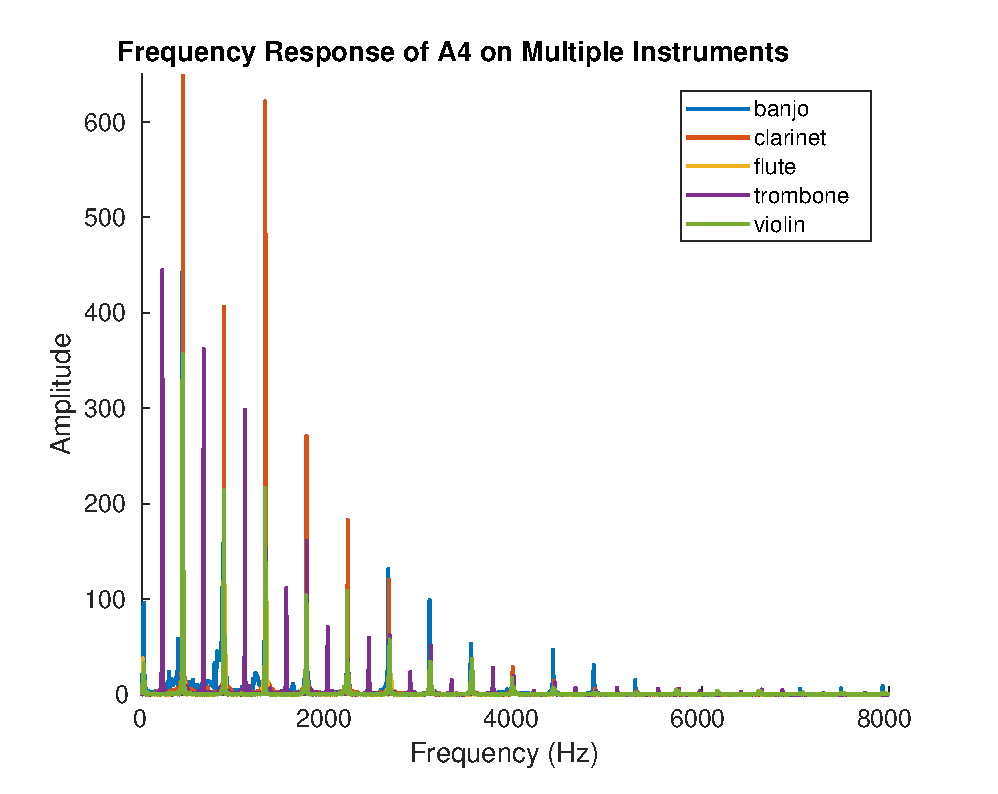
\includegraphics[width = 1.0\textwidth]{fft_all}
\end{column}
\end{columns}

\end{frame}

\begin{frame}
\frametitle{What is \textit{timbre}?}

\begin{columns}
\begin{column}{0.4\textwidth}
\begin{itemize}[label = $\blacktriangleright$]
\item However, envelope is also important\vspace{.5em}
\item In fact, a 2011 study by Heng \textit{et al.} demonstrated that cochlear implant users can differentiate between instruments when 0\% TFS is used in a music-noise chimaera\vspace{.5em}
\item Normal hearing users, however, rely primarily on TFS cues to differentiate instruments
%\item  
\end{itemize}
\end{column}
\begin{column}{0.6\textwidth}
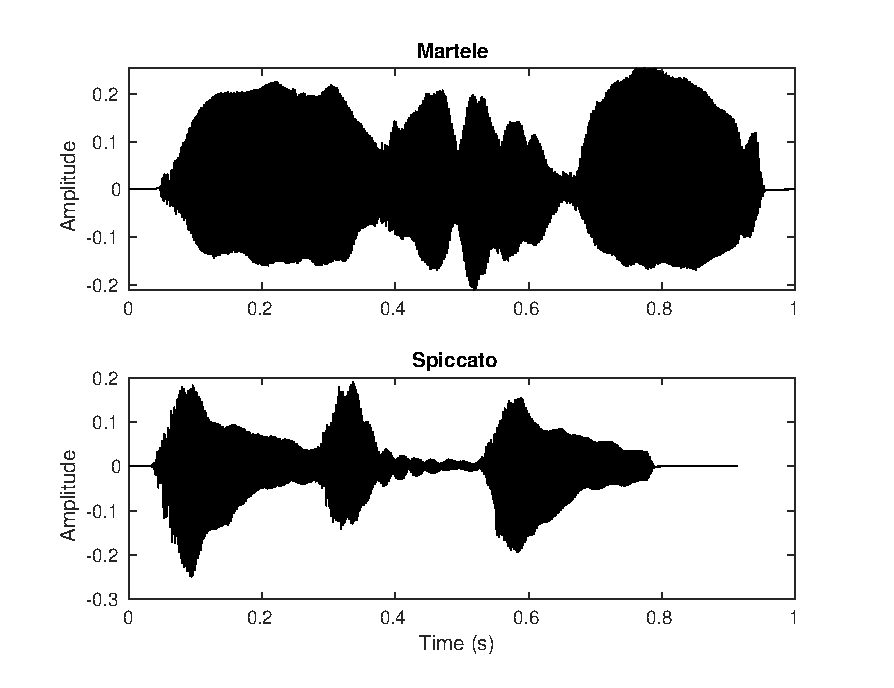
\includegraphics[width = 1.0\textwidth]{mart_spic}
\centering
Envelope cues could help us differentiate between different articulations in music, such as \href{./Audio/martele.mp3}{\textit{martele}} and \href{./Audio/spiccato.mp3}{\textit{spiccato}} played by the violin
\end{column}
\end{columns}

\end{frame}

\begin{frame}
\frametitle{Spectrotemporal Analysis}
Spectrograms are an useful tool to visualize differences in instruments. Here are a few of the stimuli I used. The sound samples were collected by the Philharmonia Orchestra in London.\\ 
\vspace{.6em}
\centering
\href{./Audio/banjo_A4_normal.mp3}{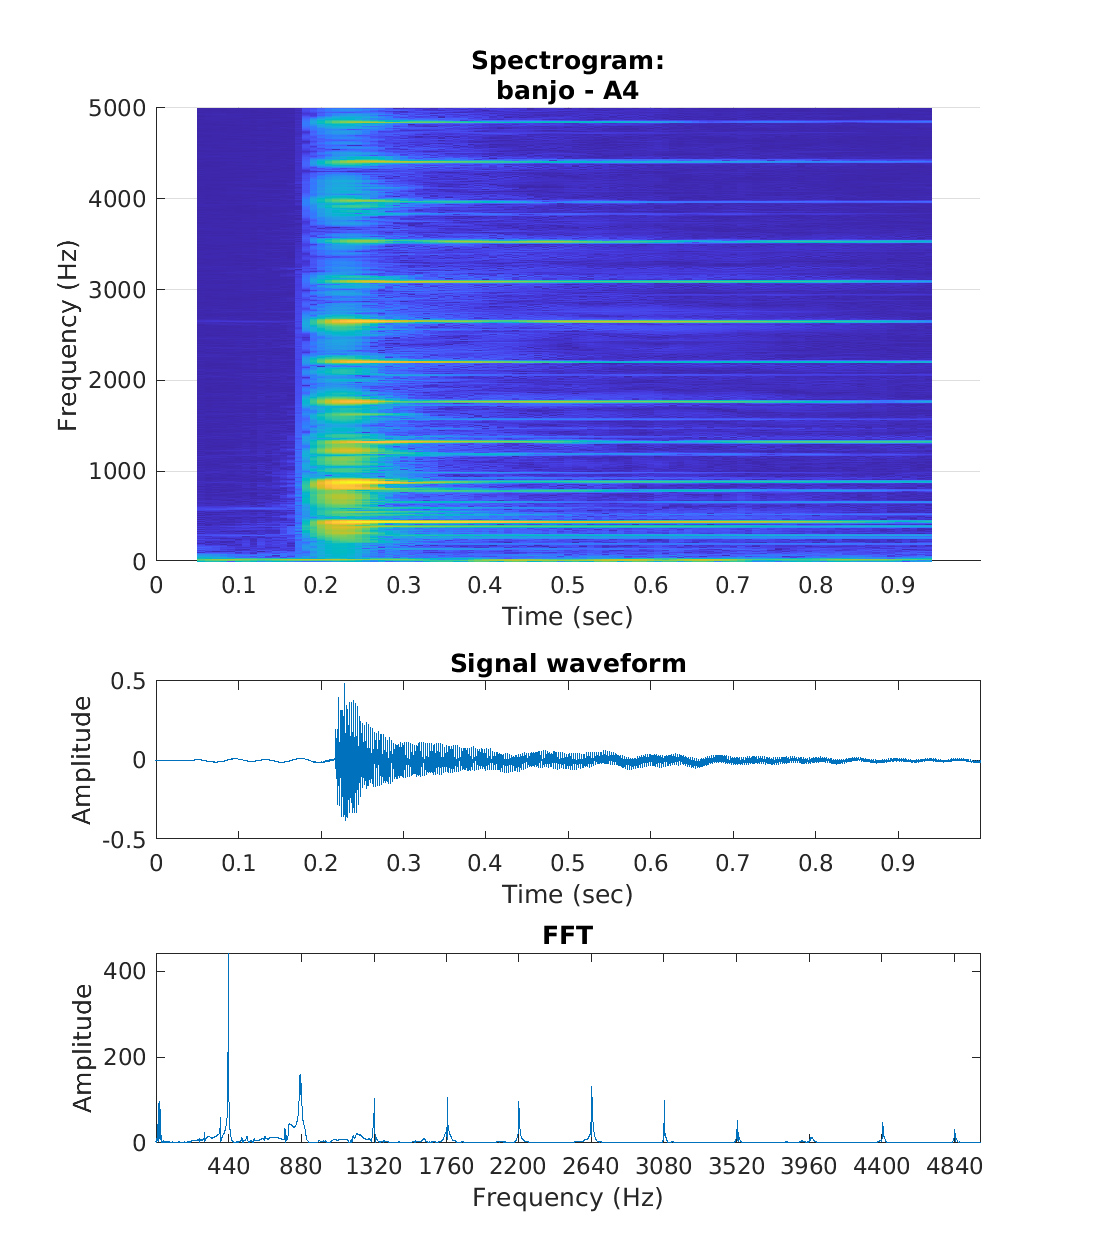
\includegraphics[height = .55\textheight]{spectrogram_banjo_normal}}
\href{./Audio/trombone_A4_normal.mp3}{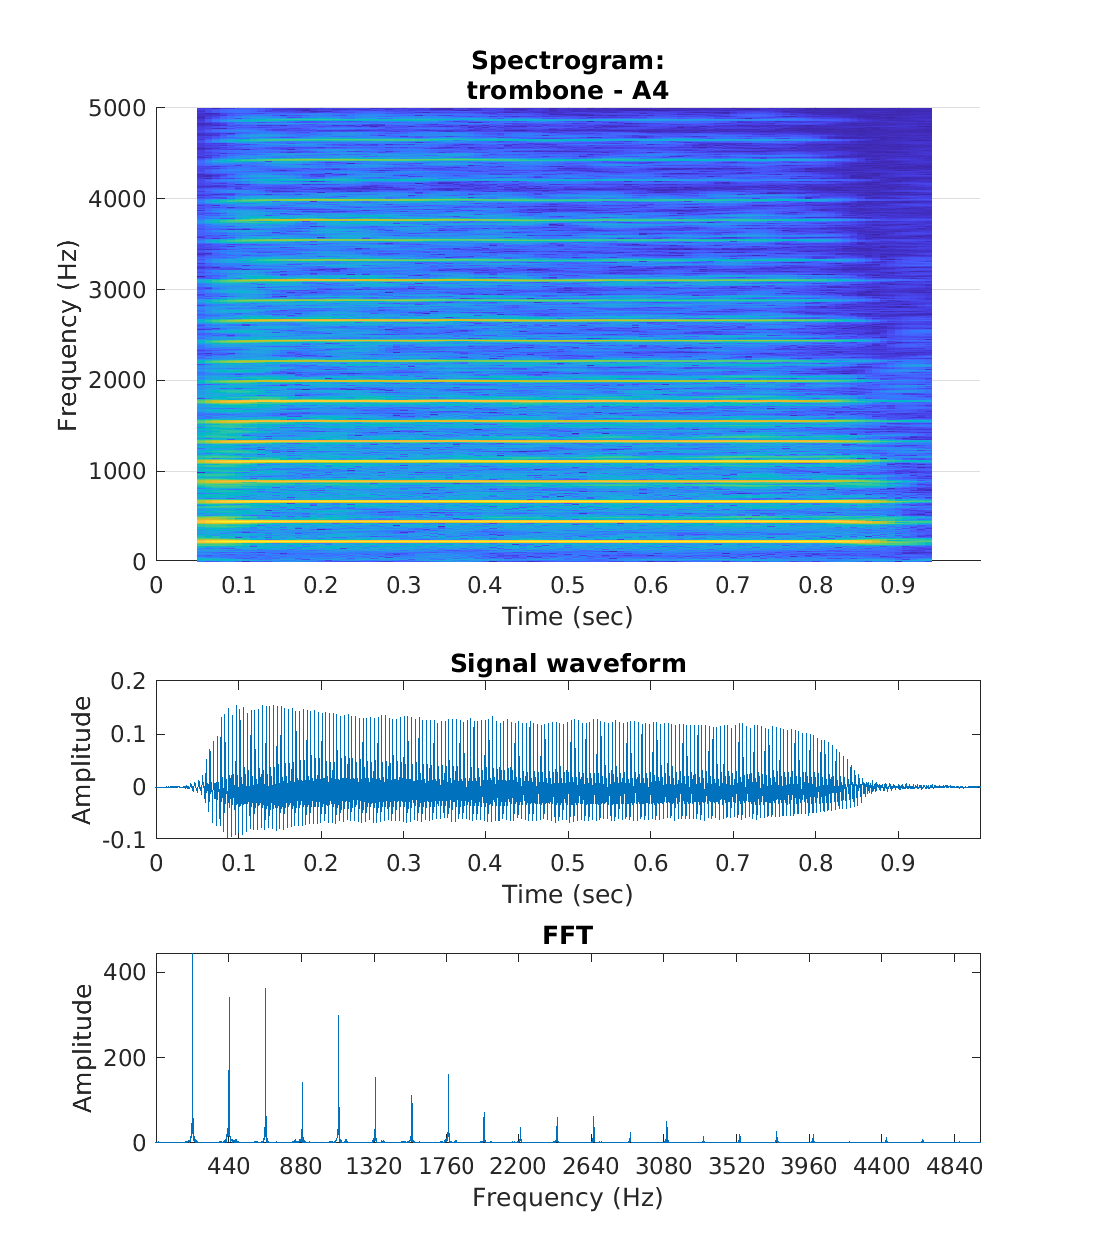
\includegraphics[height = .55\textheight]{spectrogram_trombone_normal}}
\href{./Audio/violin_A4_normal.mp3}{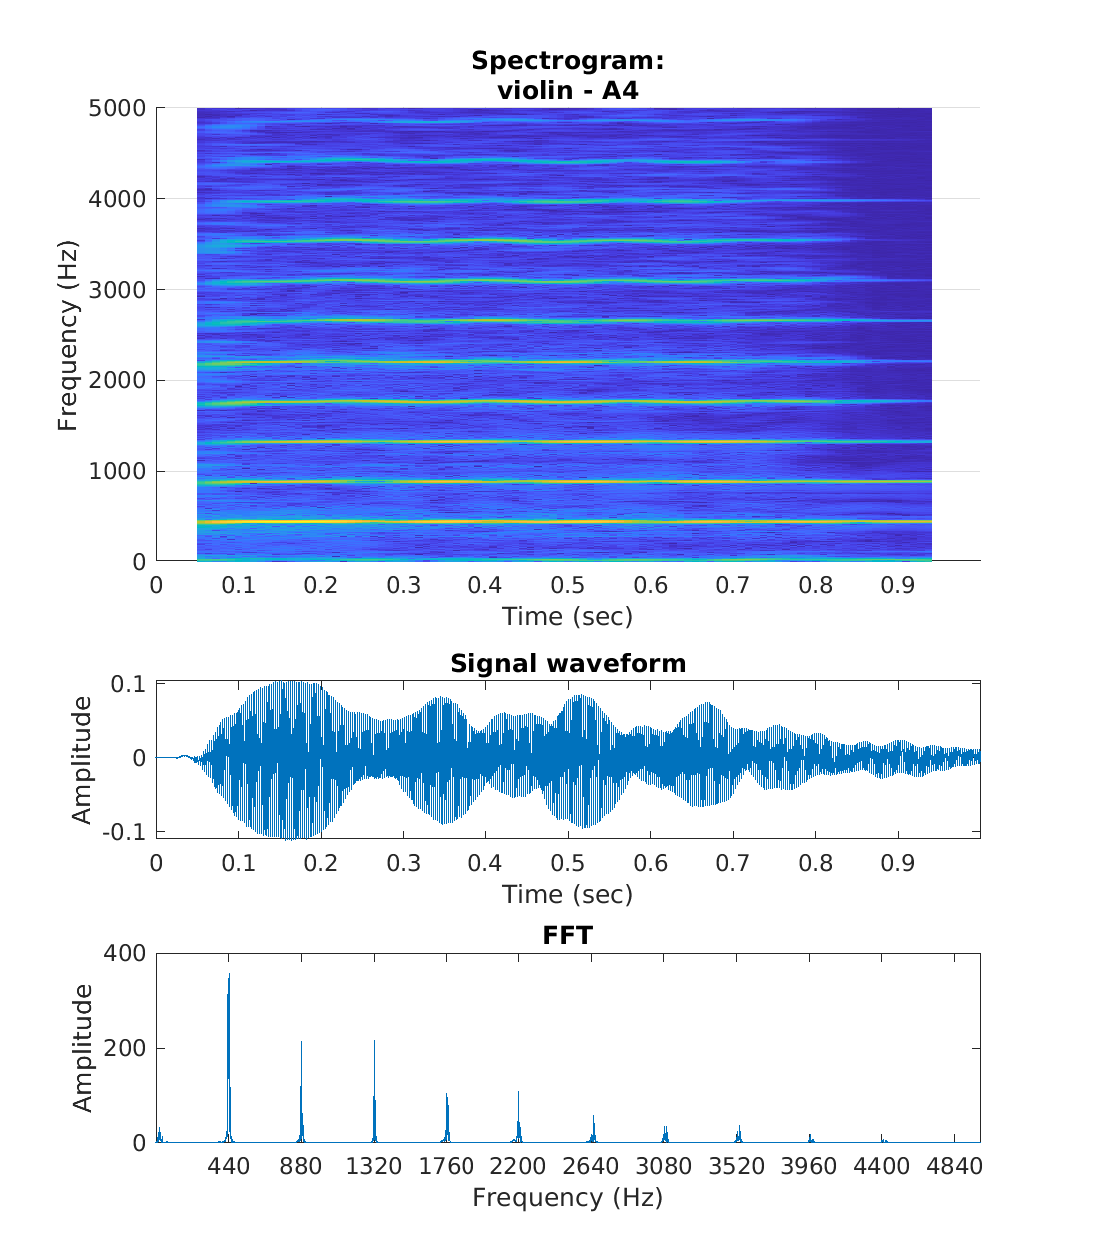
\includegraphics[height = .55\textheight]{spectrogram_violin_normal}}
\end{frame}

\begin{frame}
\frametitle{The Idea}

\textbf{\underline{Goal:}} Use a spectrally-specific framework designed to inspect the relevance of TFS and ENV in auditory nerve responses to investigate timbral coding in normal hearing and hearing impaired conditions. \vspace{1em}
\begin{itemize}
\item \textit{\underline{Aim 1:}} \textbf{Instrumental} Timbral Coding:
\begin{itemize}[label = $\blacktriangleright$]
\item Compare timbral coding differences between \textbf{banjo, clarinet, flute, trombone, violin} for a common pitch, \textbf{A4} (440 Hz)
\end{itemize}\vspace{1em}

\item \textit{\underline{Aim 2:}} \textbf{Articulation} Timbral Coding:
\begin{itemize}[label = $\blacktriangleright$]
\item Compare timbral coding differences between two articulations on the violin, \textbf{martel\'{e}} and \textbf{spiccato}
\end{itemize}

\end{itemize}
\end{frame}

\begin{frame}
\frametitle{General Methods Overview}


\centering

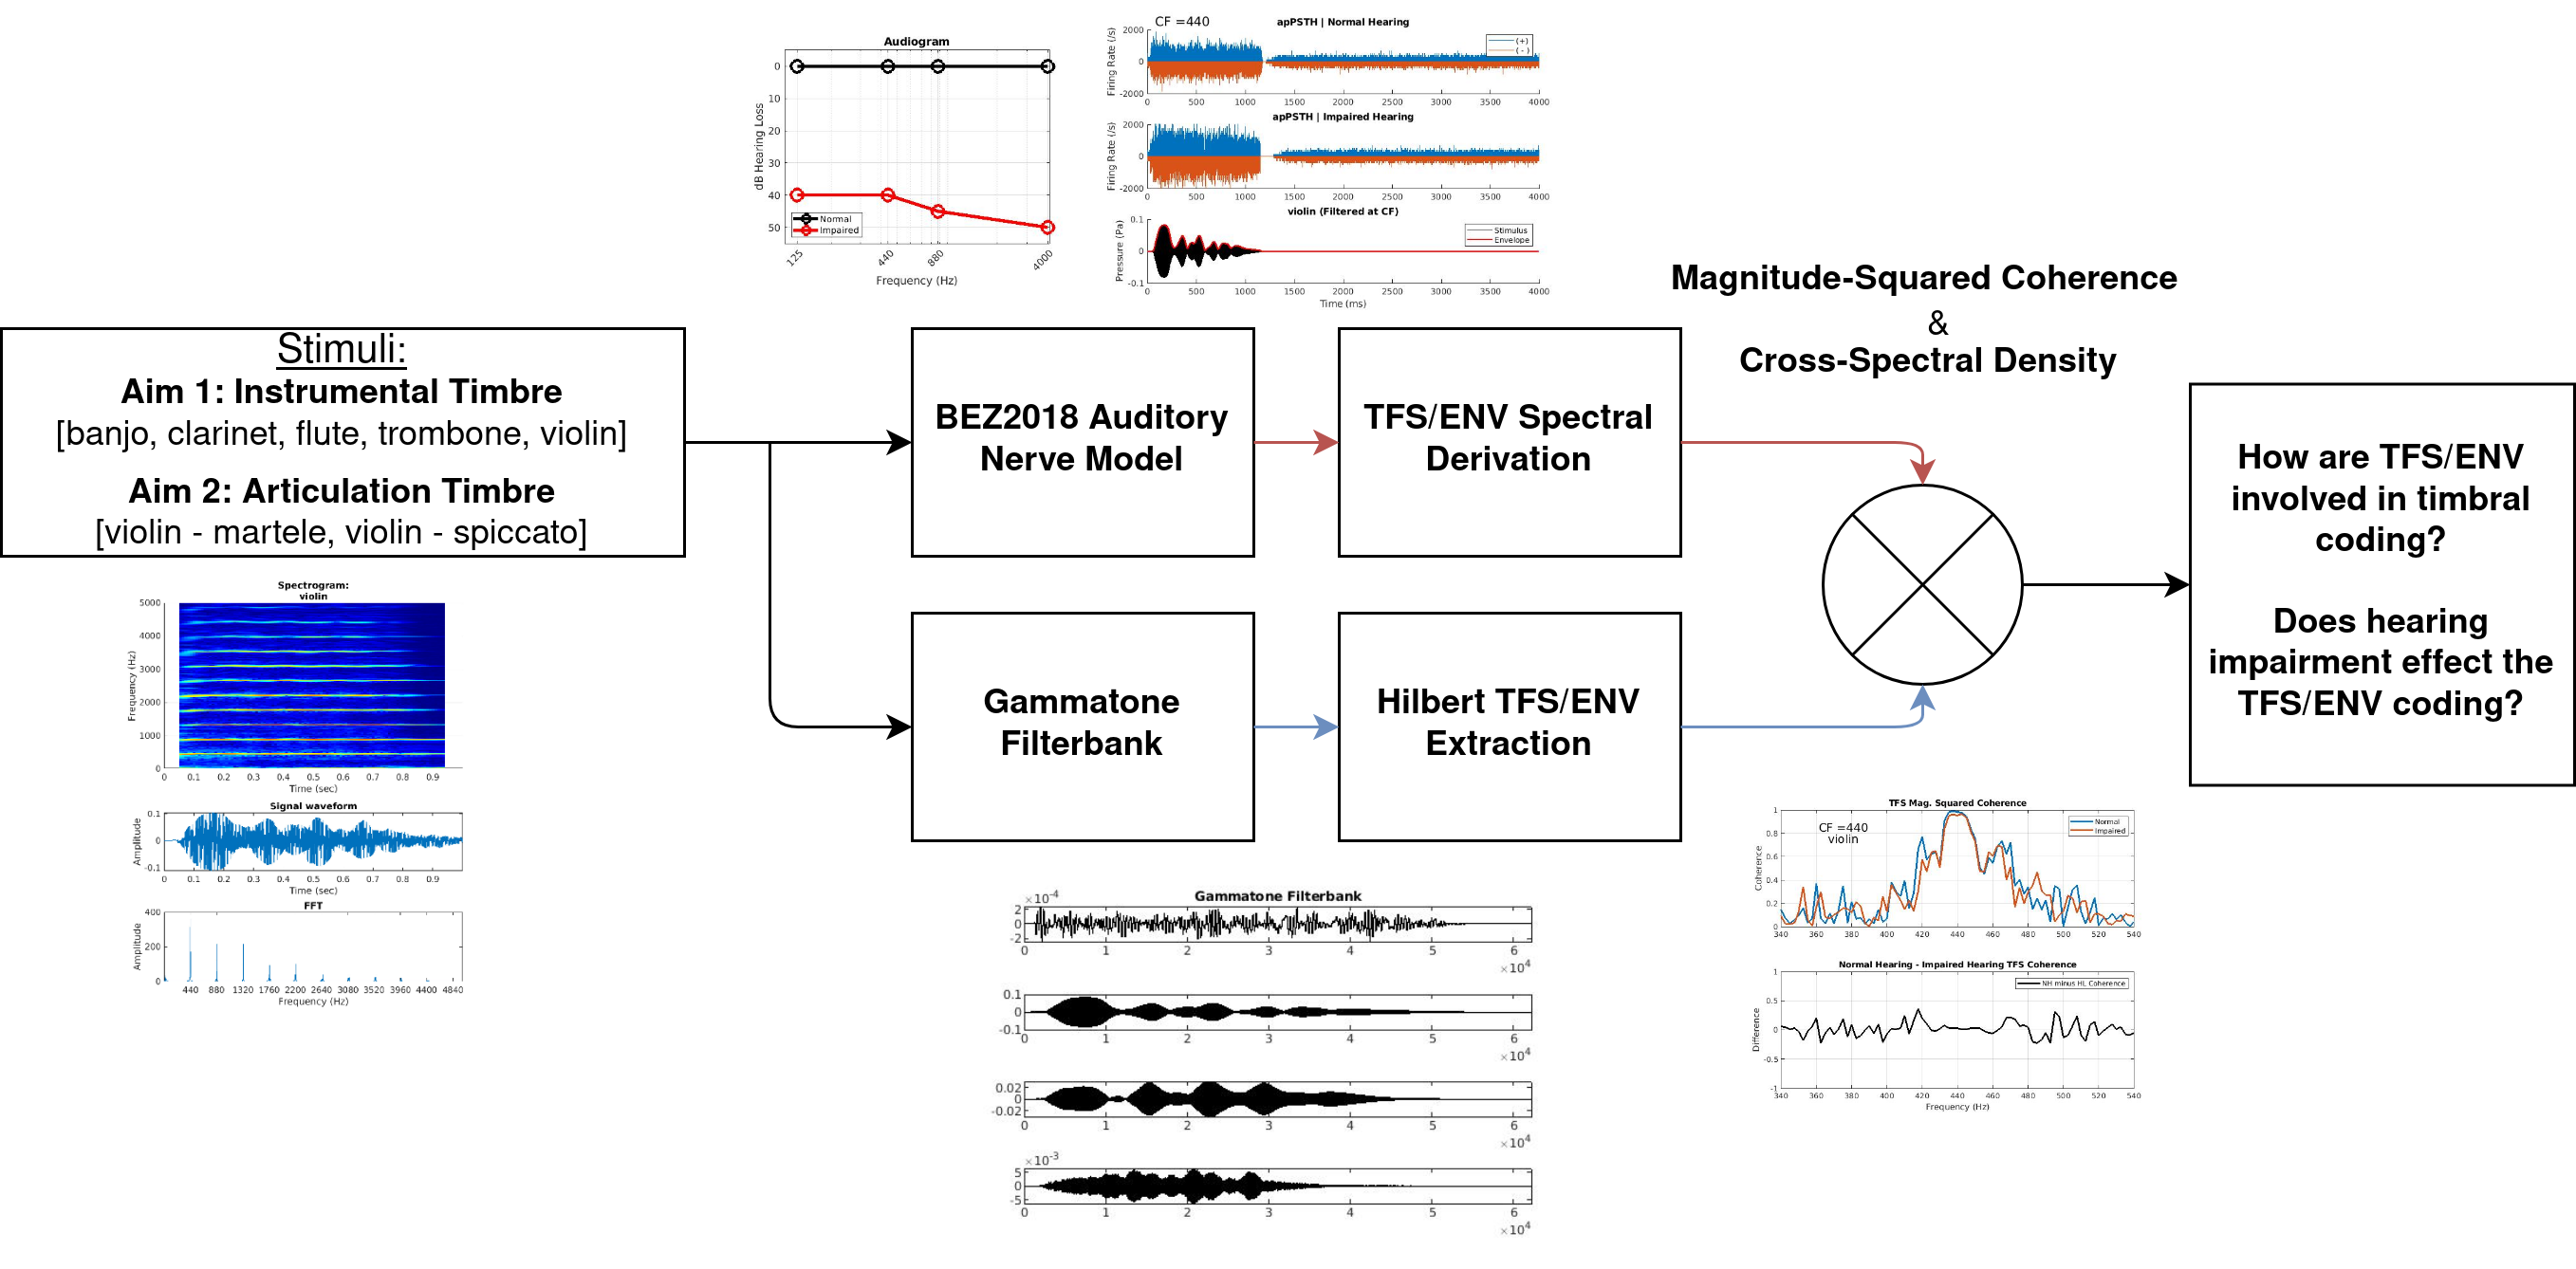
\includegraphics[height = .77\textheight]{methods_pics}

\end{frame}

\begin{frame}
\frametitle{Gammatone Filterbank and Envelope Extraction}
\begin{columns}
\begin{column}{.3\textwidth}
\begin{itemize}[label = $\blacktriangleright$]
\item Used a computationally efficient gammatone filterbank developed by Ning Ma \vspace{.5em}

\item Filtered each stimulus using same CFs used for model \vspace{.5em}

\item Extracted TFS and ENV of each channel using Hilbert analytical signal
\end{itemize}
\end{column}
\begin{column}{.7\textwidth}
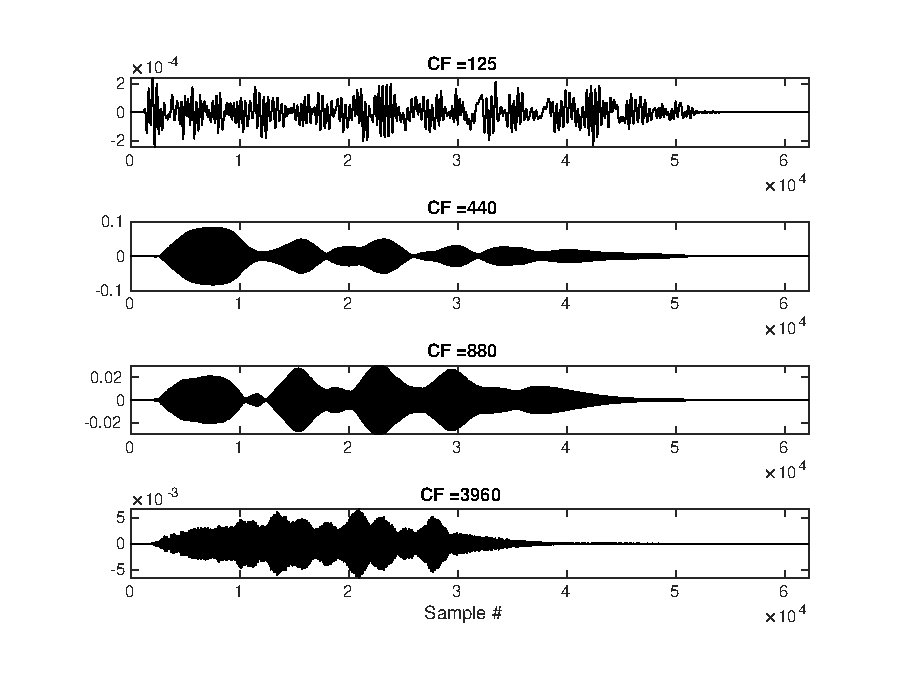
\includegraphics[width = \textwidth]{filterbank}
\end{column}
\end{columns}
\end{frame}


\begin{frame}
\frametitle{Modeling Approach}

\begin{itemize}[label = $\blacktriangleright$]
\item Using a model of the auditory nerve developed by Zilany et al. and updated by Bruce et al. in 2018, I was able to quickly collect data. \vspace{.5em}

\item This model can be run in Matlab and also has a variety of customizable parameters.\vspace{.5em}

\item I simulated auditory nerve responses at 4 different Characteristic Frequencies (CF): \\
\begin{center}
125 Hz, $F_0$ (440 Hz), $F_1$ (880 Hz), and $F_8$ (3960 Hz)
\end{center}\vspace{.5em}

\item The Organ of Corti in the cochlea can be thought of as a filterbank with filters centered around a given CF (the further down the cochlea you go, the lower the CF) 
\end{itemize}

\end{frame}

\begin{frame}
\frametitle{Modeling Approach}
This model also allowed adjustment of Outer Hair Cell and Inner Hair Cell parameters based on an audiogram. I chose hearing loss threshold shifts roughly based on data reported by Tufts et al. in a 2005 study of musical interval consonance:\vspace{1em} 

\centering
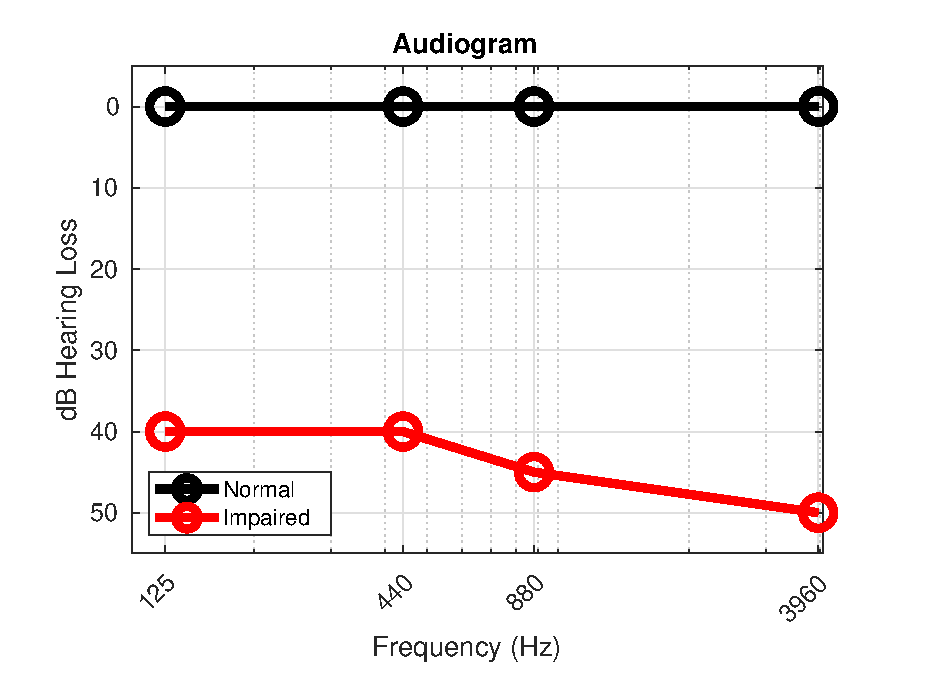
\includegraphics[width = .6\textwidth]{audiogram} 

\end{frame}

\begin{frame}
\frametitle{Modeling Approach}


\centering

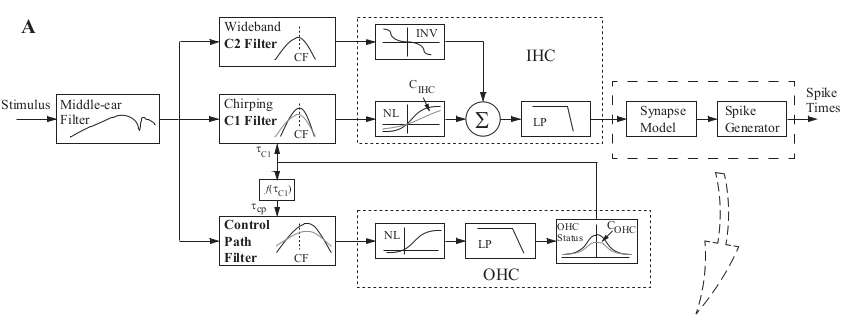
\includegraphics[width = 1\textwidth]{bruce} \vspace{.5em}
 
A schematic of the original Zilany Model. Sound stimulus goes in, spike train comes out. 

\end{frame}


\begin{frame}
\frametitle{Model Parameters and Implementation}
\textbf{Using BEZ2018 Model:}\vspace{.5em}

\begin{itemize}
\item \textbf{\underline{Parameters:}}
\begin{itemize}[label = $\blacktriangleright$]
\item CF (Hz) = 125, 440, 880, 3960
\item Repetitions/CF = 75
\item Spont. Rate = 70
\item Abs and Baseline mean relative refrac. period = 0.6 ms
\item IHC/OHC health = set by \texttt{fitaudiogram2}
\item Species = Human - Shera tuning
\item Fractional Gauss. noise type = 0 (fixed)
\item Power-law functions = 0 (approximate)
\item \textbf{Spike time resolution = 10} $\mu$s
\end{itemize}\vspace{.5em}

\item \textbf{\underline{Other Details:}}
\begin{itemize}[label = $\blacktriangleright$]
\item Compensated for threshold shift in Hearing Loss condition by increasing stimulus gain by mean threshold shift (43.75 dB)
\end{itemize}
\end{itemize}

\end{frame}

\begin{frame}
\frametitle{Model Output}
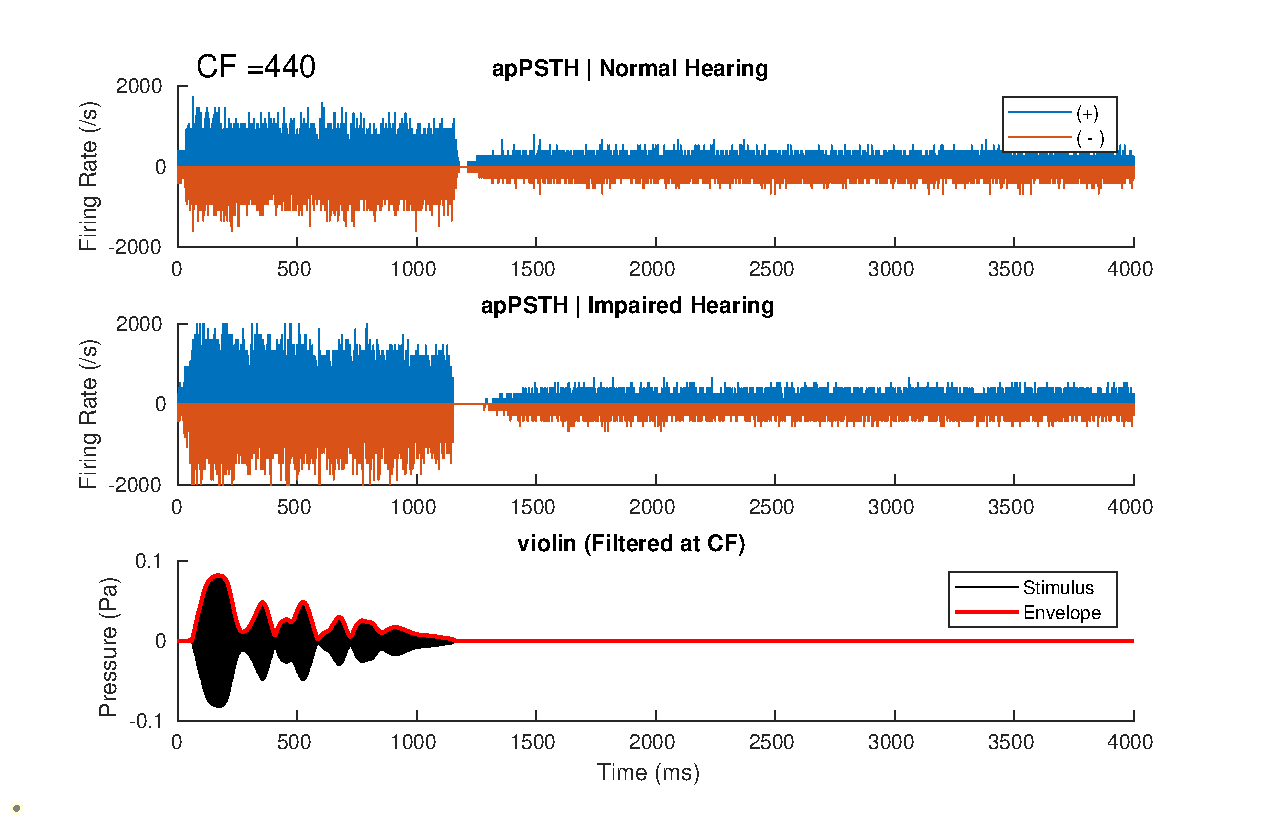
\includegraphics[width = .88\textwidth]{apPSTH_violin}
\end{frame}

\begin{frame}

\frametitle{apPSTH Analysis}

Used the rationale developed by Parida et al. to compute $s(t)$ and $\phi (t)$ and their spectrograms corresponding to ENV and TFS characteristics:\vspace{1em}

\underline{ENV-related response, the \textit{sum} PSTH (polarity-tolerant):}\\
\begin{center}
\scalebox{1.2}{
$s(t) = \frac{p(t)+n(t)}{2}$}
\end{center}

\underline{TFS-related response to PSTH (polarity-sensitive):}\\
\begin{center}

$\phi (t) = \sqrt{2} \times rms[d(t)] \times \cos[\angle d(t)]$\\
\end{center}

Where:
 \begin{center}
 \scalebox{1.2}{
 $d(t) = \frac{p(t)-n(t)}{2}$}
\end{center}

\end{frame}

\begin{frame}

\frametitle{Measuring the ``strength" of TFS/ENV Coding}

The coding ``strength" of the ENV and TFS nerve responses can then be assessed using either cross-spectral density or coherence with the Hilbert ENV or TFS. Magnitude-squared Coherence, $C_{xy}(f)$, is a nice way to compare these, since it is essentially a normalized cross-spectral density:\vspace{2em}

\begin{center}
\scalebox{1.5}{
$C_{xy}(f) = \frac{|P_{xy}(f)^2|}{P_{xx}(f)P_{yy}(f)}$}
\end{center}

\end{frame}

\begin{frame}

\frametitle{ENV and TFS Coherence Across Instruments}

\begin{columns}
\begin{column}{0.55\textwidth}
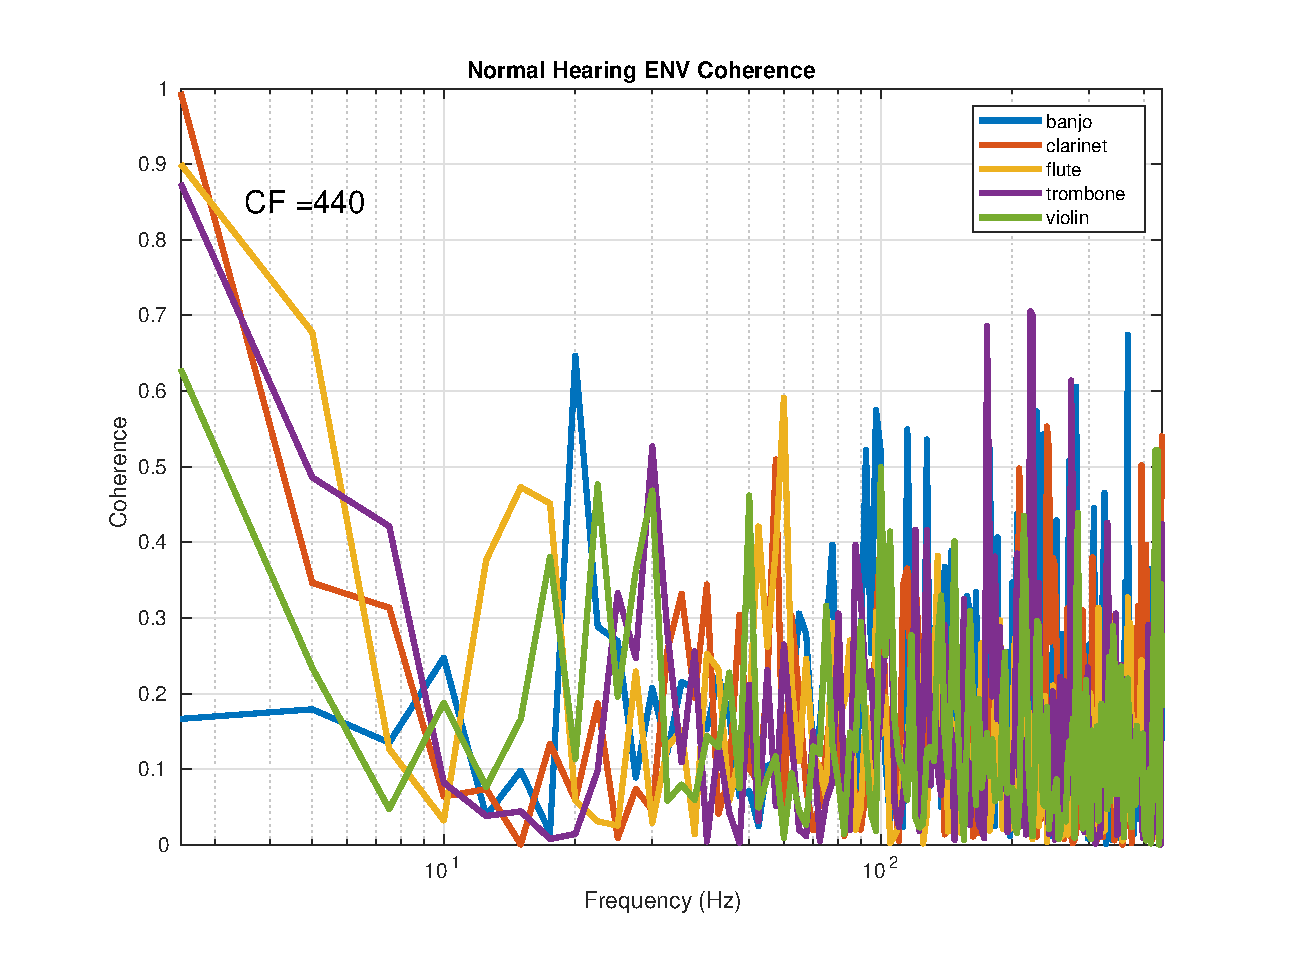
\includegraphics[scale = .4]{all_ENV_coherence_440}
\end{column}
\begin{column}{0.56\textwidth}
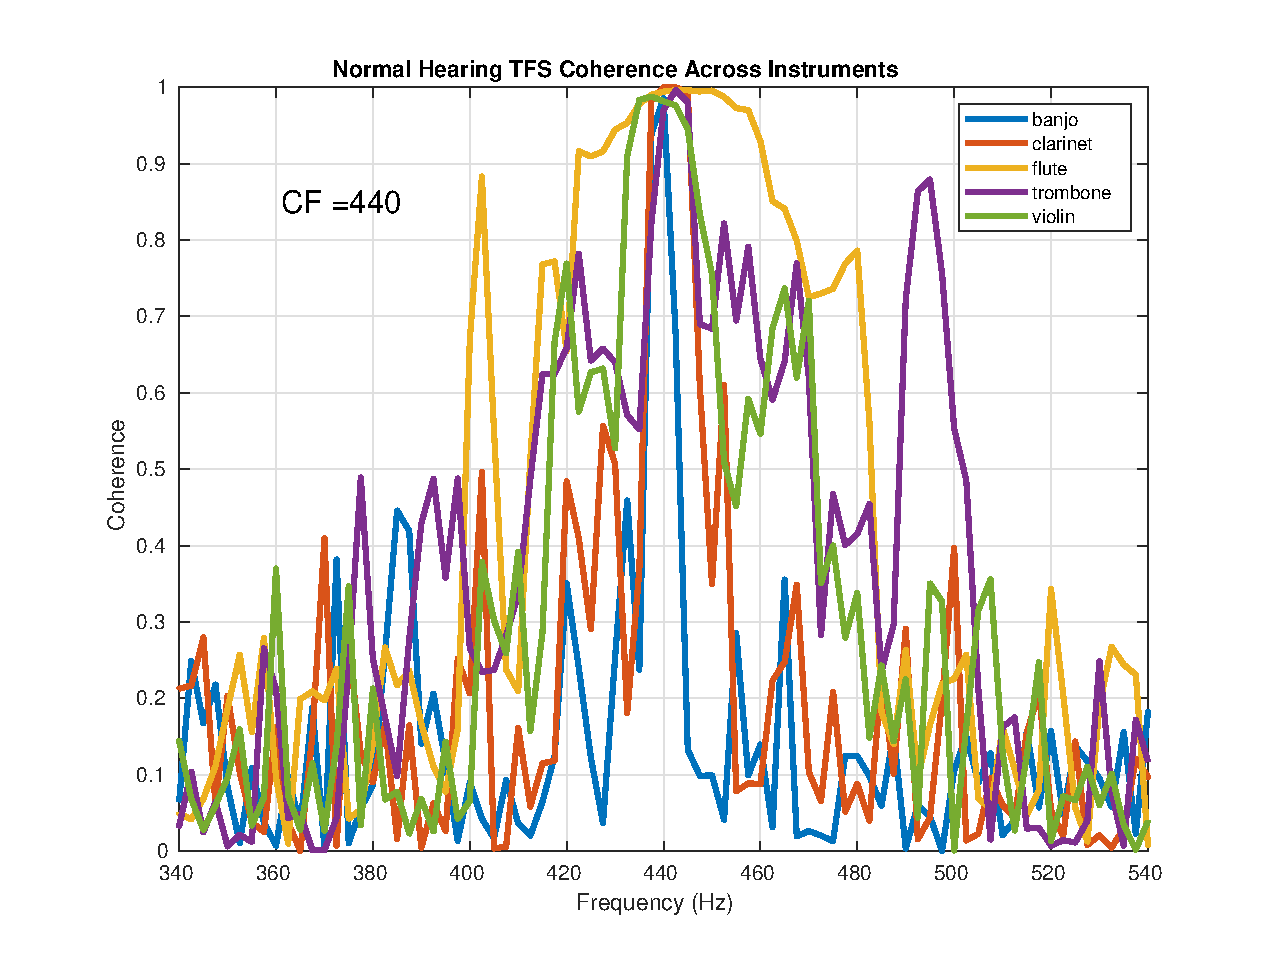
\includegraphics[scale = .4]{all_TFS_coherence_440}
\end{column}
\end{columns}

\end{frame}


\begin{frame}

\frametitle{ENV and TFS Coherence Across Instruments}

\begin{columns}
\begin{column}{0.55\textwidth}
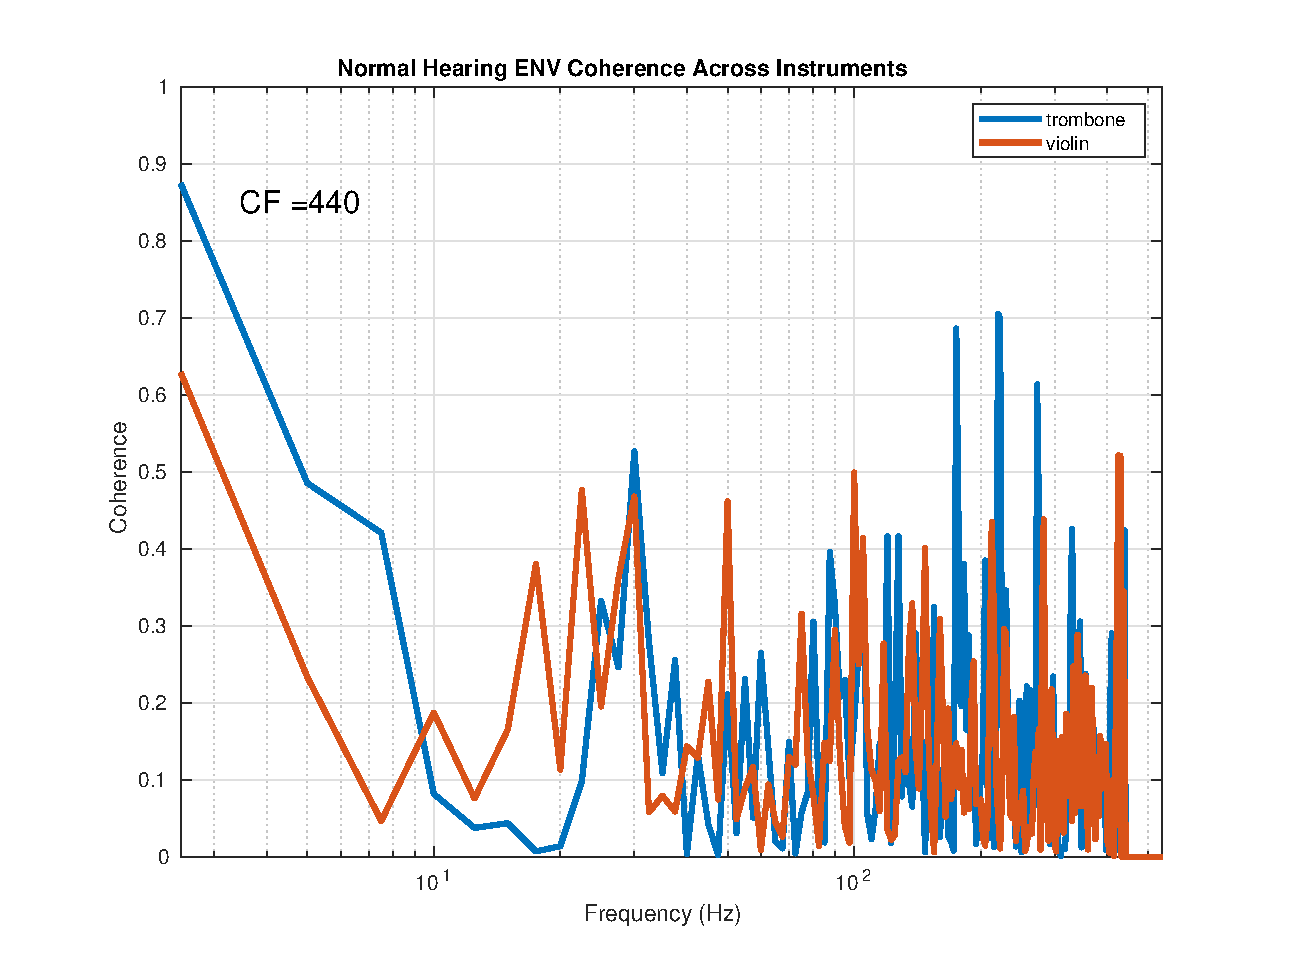
\includegraphics[scale = .4]{trombone_violin_ENV_coherence_440}
\end{column}
\begin{column}{0.56\textwidth}
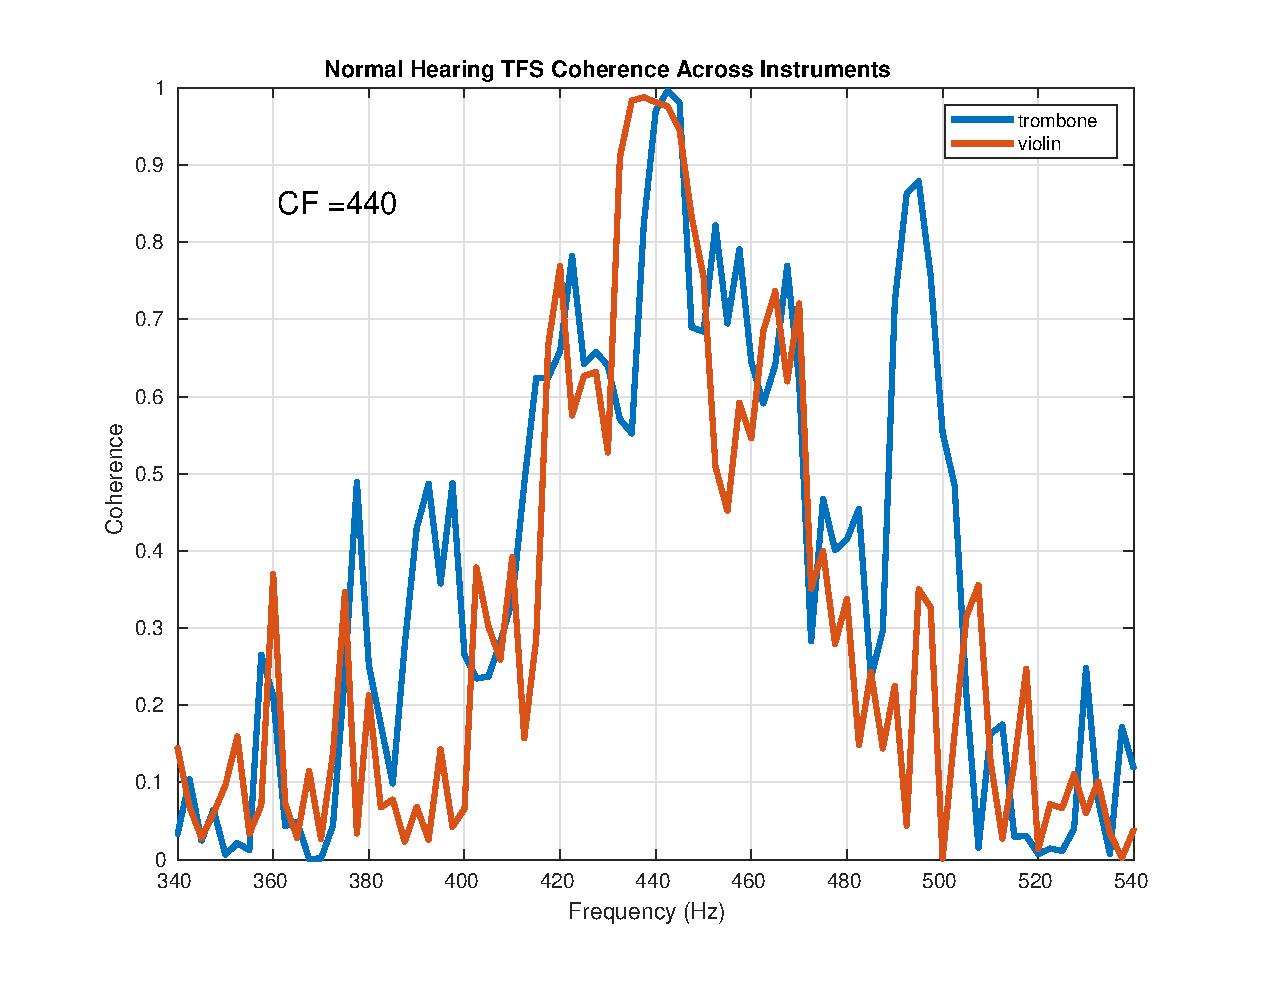
\includegraphics[scale = .4]{trombone_violin_TFS_coherence_440}
\end{column}
\end{columns}
\end{frame}

\begin{frame}
\frametitle{Effects of Hearing Loss on ENV and TFS Coherence} 

\begin{columns}
\begin{column}{0.55\textwidth}
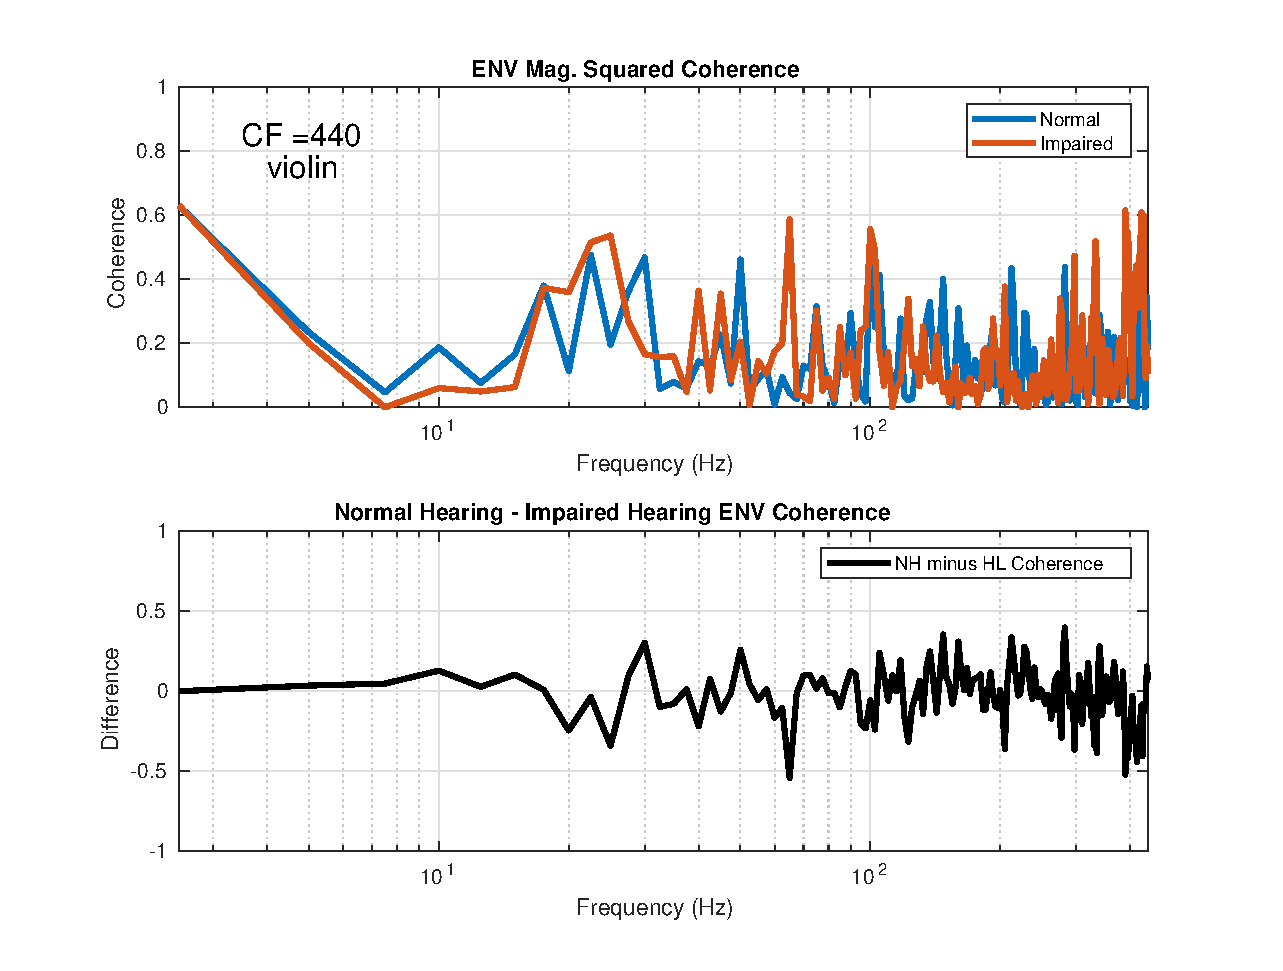
\includegraphics[scale = .4]{violin_ENV_COH_440}
\end{column}
\begin{column}{0.56\textwidth}
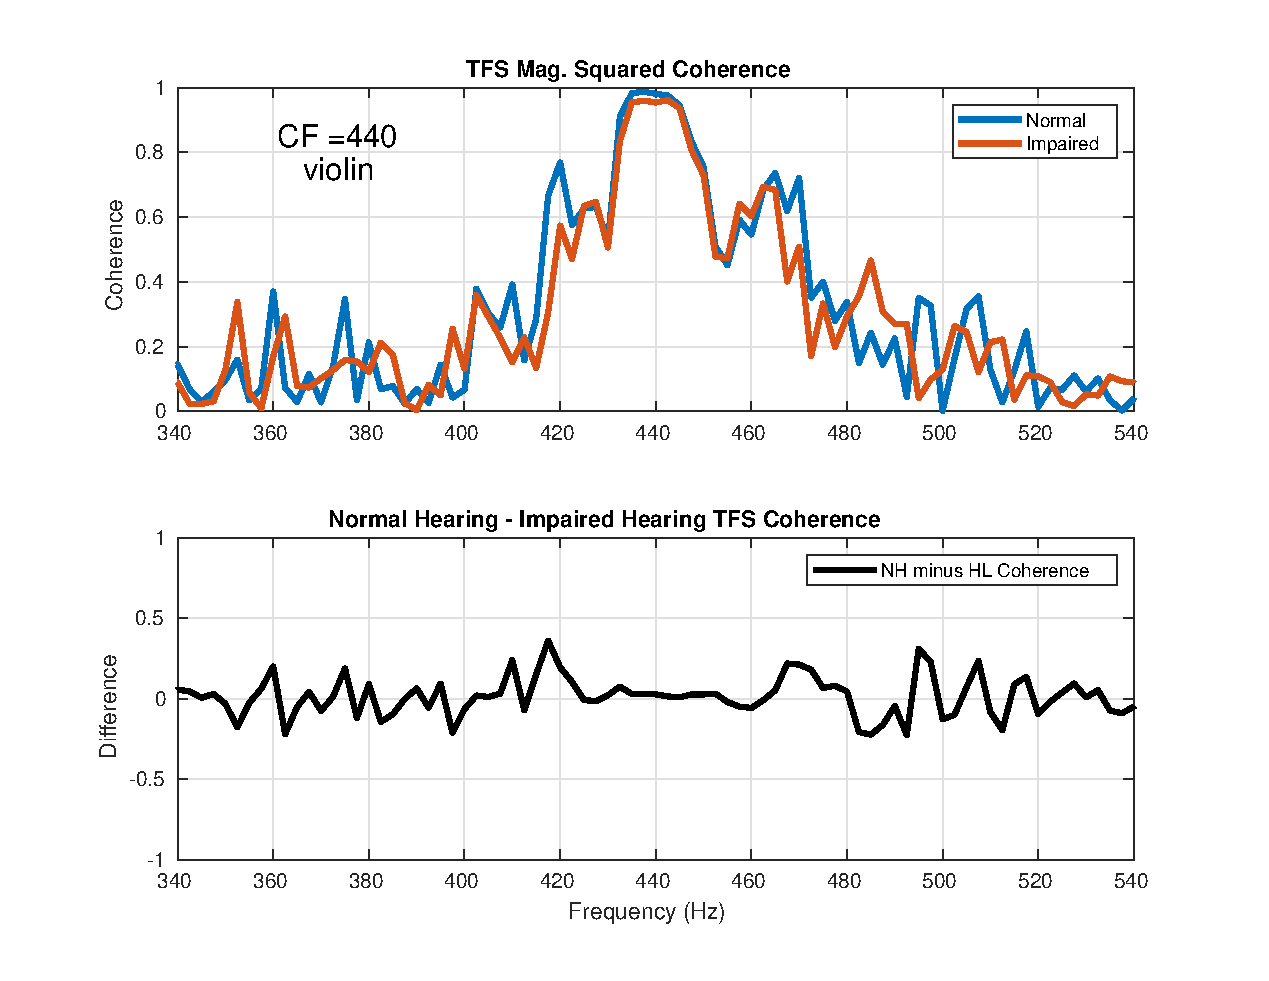
\includegraphics[scale = .4]{violin_TFS_COH_440}
\end{column}
\end{columns}

\end{frame}

\begin{frame}
\frametitle{Effects of Hearing Loss on ENV and TFS Coherence} 

\begin{columns}
\begin{column}{0.55\textwidth}
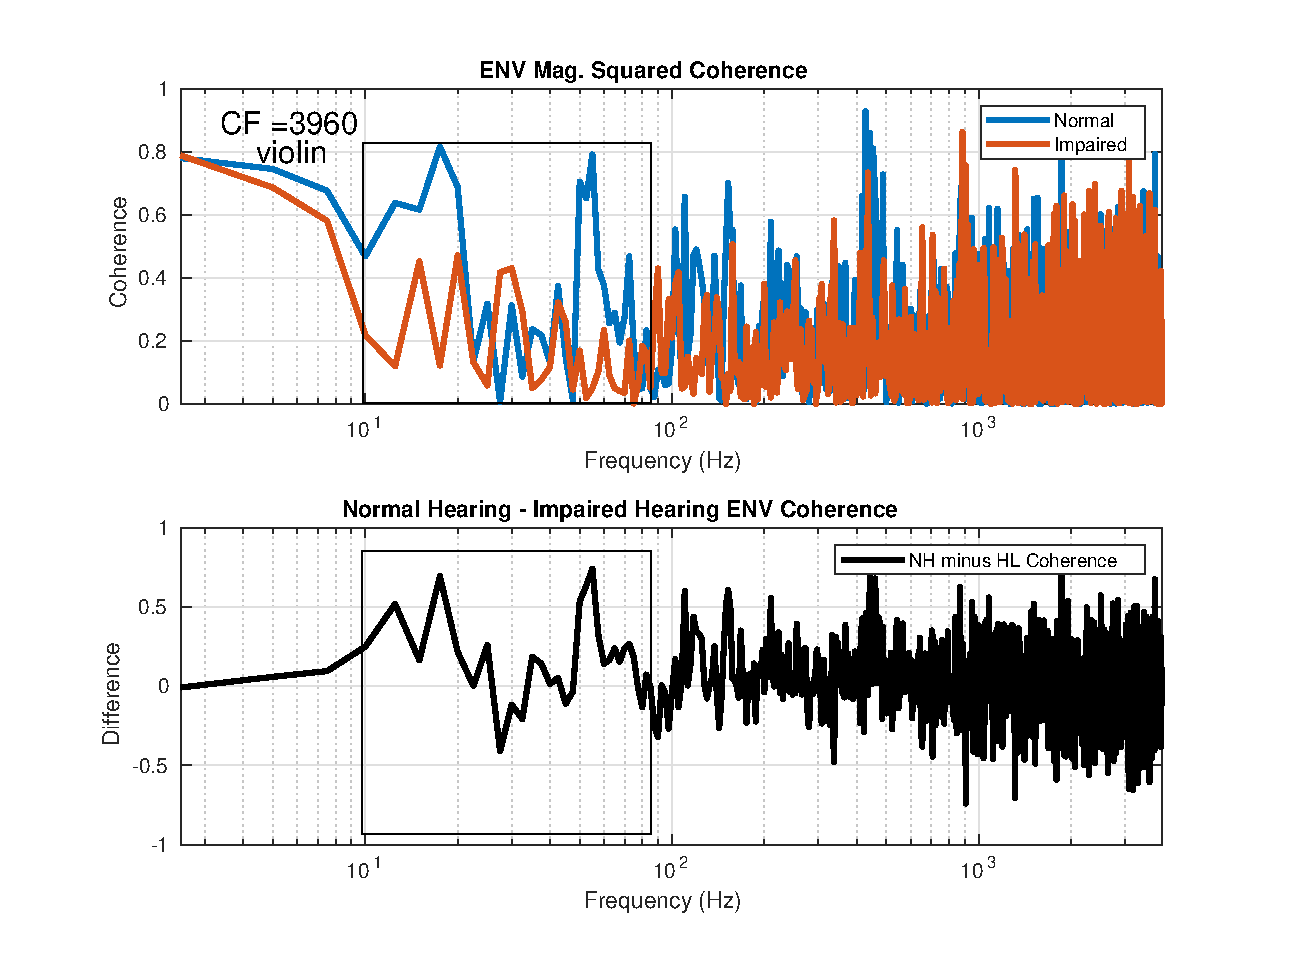
\includegraphics[scale = .4]{violin_ENV_COH_3960}
\end{column}
\begin{column}{0.56\textwidth}
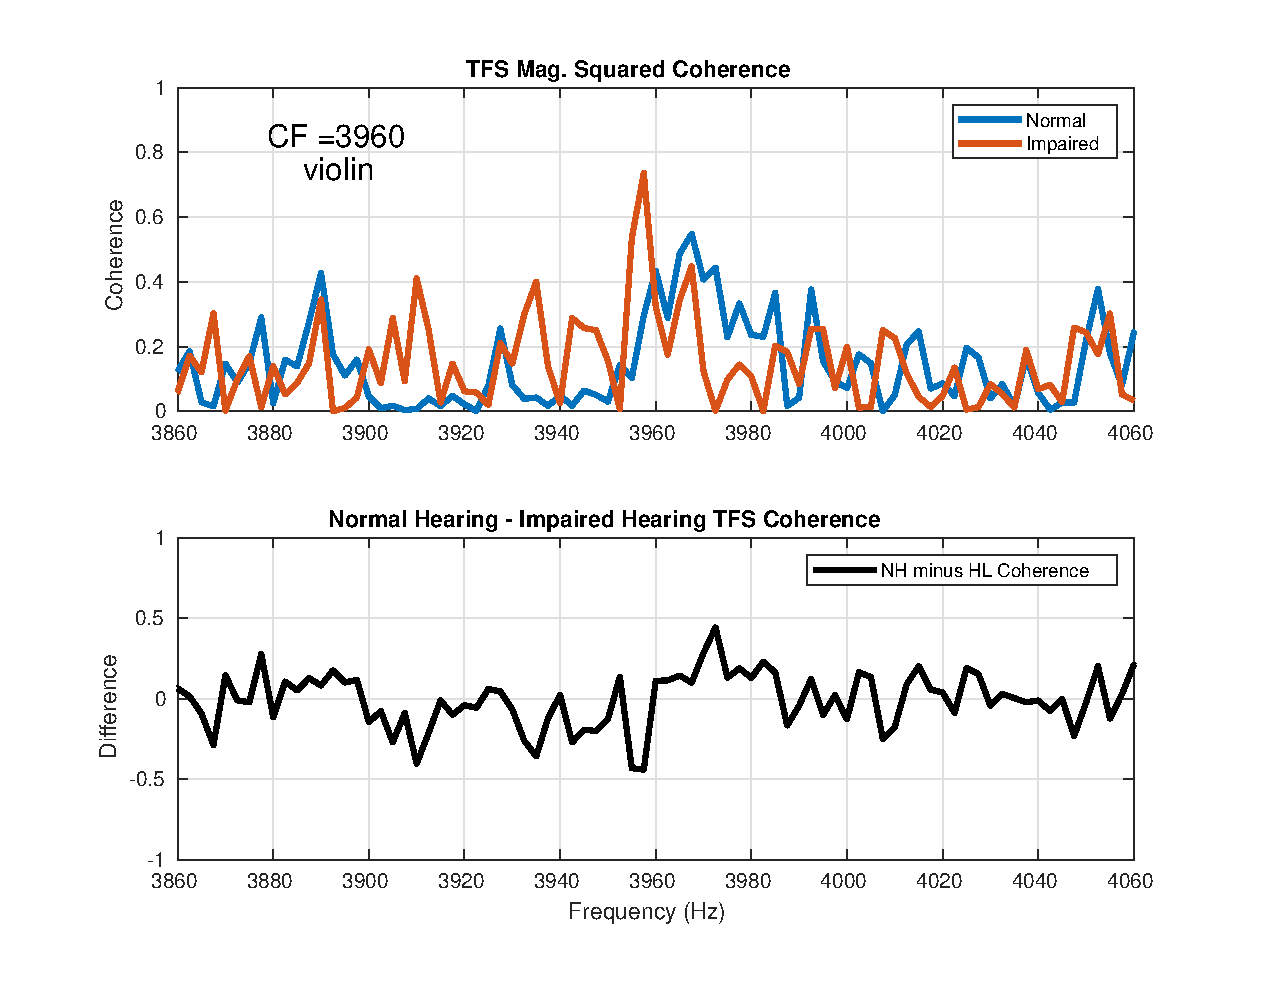
\includegraphics[scale = .4]{violin_TFS_COH_3960}
\end{column}
\end{columns}

\end{frame}

\begin{frame}
\frametitle{Hearing Loss May Effect Timbral Coding of ENV in Articulation} 

\begin{columns}
\begin{column}{0.55\textwidth}
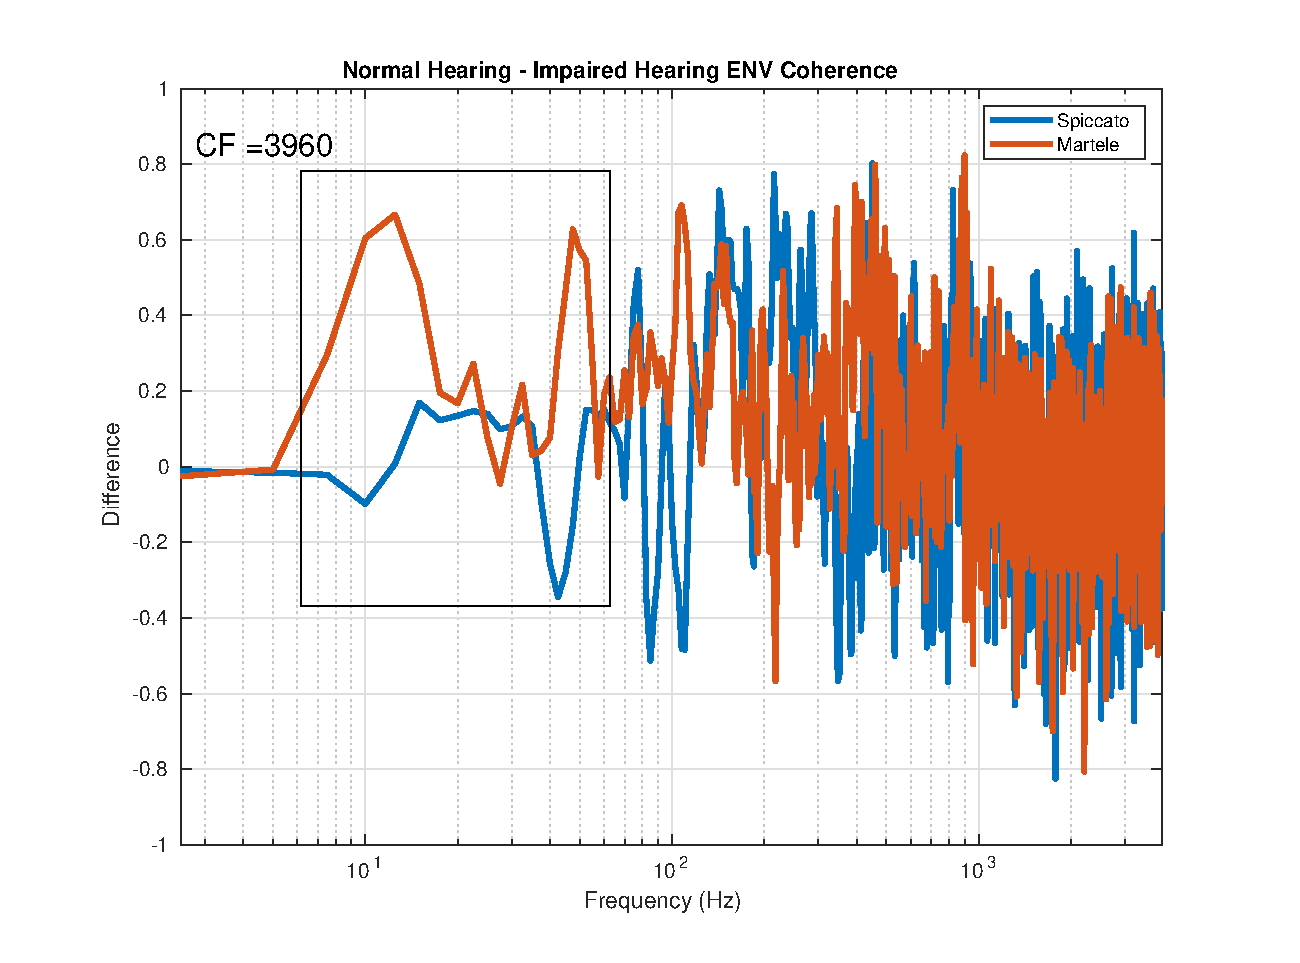
\includegraphics[scale = .4]{martele_spiccato_ENV_3960}
\end{column}
\begin{column}{0.56\textwidth}
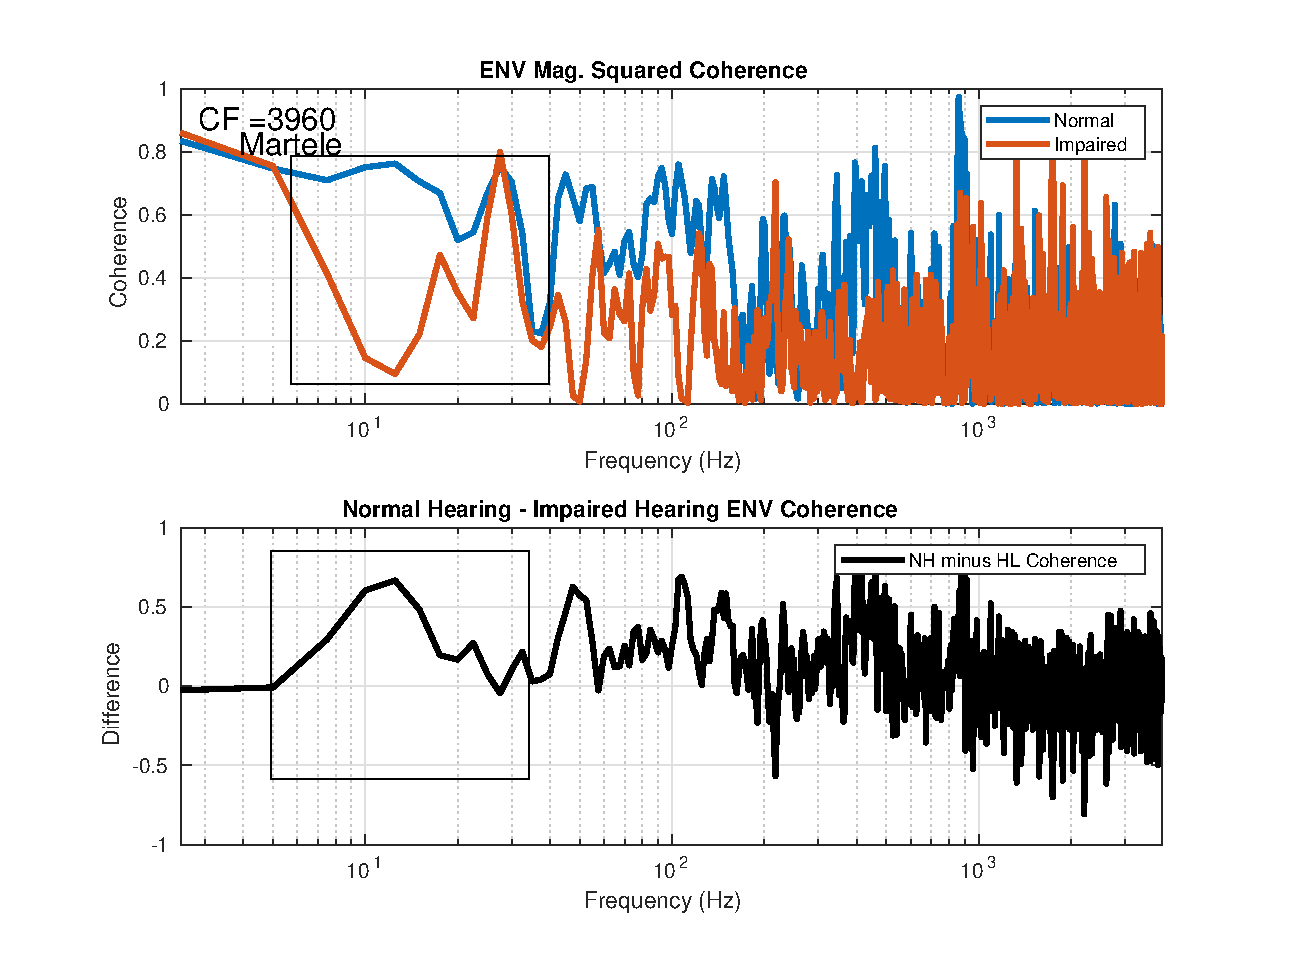
\includegraphics[scale = .4]{martele_ENV_diff}
\end{column}
\end{columns}

\end{frame}


\begin{frame}
\frametitle{Hearing Loss May Not Affect Timbral Coding of TFS in Articulation} 

\begin{columns}
\begin{column}{0.55\textwidth}
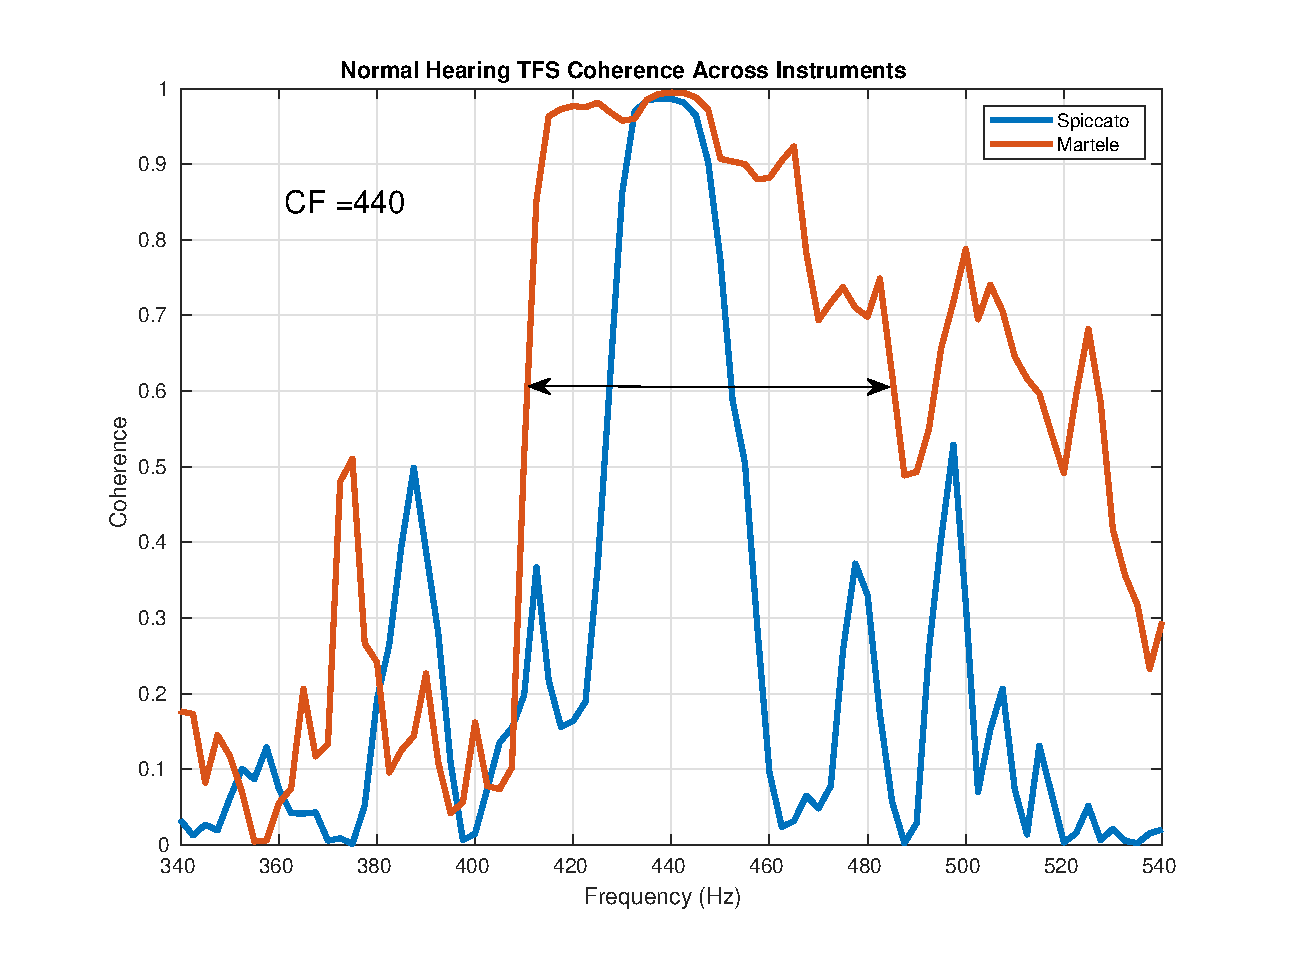
\includegraphics[scale = .4]{martele_spiccato_TFS_440}
\end{column}
\begin{column}{0.56\textwidth}
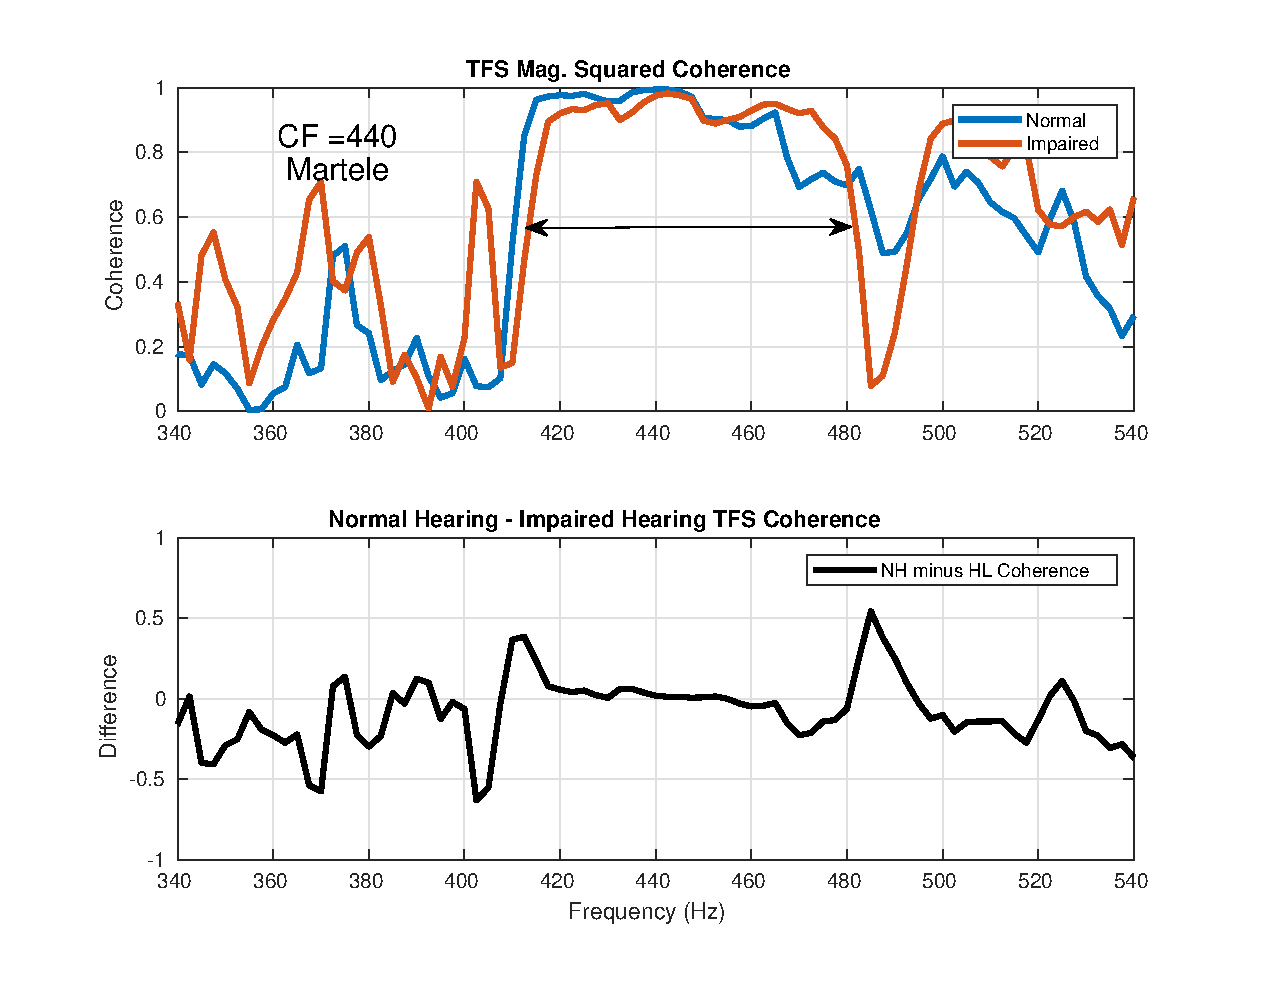
\includegraphics[scale = .4]{martele_TFS_diff_440}
\end{column}
\end{columns}

\end{frame}

\begin{frame}
\frametitle{Conclusion}
\begin{itemize}[label = $\blacktriangleright$]
\item A framework was designed to investigate TFS/ENV coding of timbre \vspace{.5em}
\item The spectral composition of instrumental tones and articulation is non-trivial
\vspace{.5em}
\item Understanding the way we perceive sound beyond the auditory periphery is likely very important in solidifying the relevance of TFS/ENV in timbral perception
\vspace{.5em}
\item Even at the peripheral level, it appears coding of ENV and TFS may be affected by hearing loss
\vspace{.5em}
\item The framework used to analyze ENV/TFS coding can be extended to \textit{in vivo} auditory nerve measurements or non-invasive measures collected using EEG, so could be fun to try this in the lab
\end{itemize}

\end{frame}


\begin{frame}

\frametitle{Future Considerations/Work}

\begin{itemize}[label = $\blacktriangleright$]
\item There are a lot of coherence plots I can generate with my code...but how to sort through them
\vspace{.5em}
\item These timbral coding effects vary from instrument to instrument so finding a unifying, non-noisy, metric to measure across multiple conditions would be helpful
\vspace{.5em}
\item Other parameters to mess with? Any shortcomings of model to consider?
\vspace{.5em}
\item How can I reduce variance in the coherence? Multi-tapered Coherence? 
\vspace{.5em}
\item Worth studying further? Other ideas of things to look at?
\end{itemize}

\centering
\vspace{2em}
\textbf{Questions/Other points of Discussion??}
\end{frame}

\end{document}